\documentclass{beamer}
\usetheme{Madrid}
\usepackage[utf8]{inputenc}
\usepackage[ruled,linesnumbered]{algorithm2e}
\usepackage{amsmath,amsthm,amssymb,amsfonts}
\usepackage{mathtools}
\usepackage{booktabs}       % professional-quality tables
\usepackage{graphicx}
\usepackage{array}
\DeclareMathOperator*{\argmin}{argmin}
\DeclareMathOperator*{\argmax}{argmax}

\title[]{Empirical Assessment of HMM and HDP-HSMM Methods}
\subtitle{TTIC 31150 - Robotics}
\author[Lam, Sawhney, Yoo]{A. Lam \and K. Sawhney \and J. Yoo}

\date[June 2019]{June 2019}

\begin{document}

\frame{\titlepage}

\begin{frame}
\frametitle{Outline}
    \begin{enumerate}[I]
        \item Introduction
        \item HMM, HSMM \& HDP-HSMM
        \item Data Generation
        \item Empirical Results
        \item Conclusion
    \end{enumerate}
\end{frame}


\begin{frame}
\frametitle{Introduction - Problem Statement}
    \begin{itemize}
        \item Algorithms to estimate the most likely sequence of hidden states from observations in a \textbf{HMM rely on the Markov assumption} -- that future states are conditionally independent of past states given the present state
        \item The most popular method for estimating these states involves evaluating conditional likelihoods using the forward-backward algorithm and then inferring the most likely sequence of hidden states using the Viterbi algorithm
        \item However, it has been suggested that \textbf{the Markov assumption need not be strictly met} for these techniques to generate reasonably accurate estimates of hidden state sequences
    \end{itemize}
\end{frame}

\begin{frame}
    \frametitle{Introduction - Analysis}
        \begin{itemize}
            \item We sought to \textbf{empirically test this proposition} on the problem of estimating an agent's path in a GridWorld setting
            \item Specifically, we \textbf{simulate agent pathways} under a variety of settings that differ in grid size, placement of obstacles, and transition mechanism, including settings which violate the Markov assumption implicit to traditional HMMs
            \item Hierarchical Dirichlet Process Hidden Semi-Markov Models (\textbf{HDP-HSMMs}) are a Bayesian non-parametric approach to estimating hidden state sequences, where transition, emission and initial state distribution priors are not defined by the user. It is expected that these models will outperform HMMs in non-Markovian settings by better capturing these effects
        \end{itemize}
    \end{frame}

\begin{frame}
    \frametitle{HMM \& HSMM}
        A HMM consists of two sequences:
        \begin{itemize}
          \item A \textbf{state sequence} $z = \{z_1, z_2, \dots, z_T\}$ where $z_t$ is the state at timestep $t$ which takes a value from a state space $\mathcal{Z}$ that is assumed to be static and finite for $t = 1, 2, \dots, T$.
          \item An \textbf{observation (or emission) sequence} $x = \{x_1, x_2, \dots, x_T\}$ where $x_t$ is the observation at timestep $t$ from an observation space $\mathcal{X}$ that is assumed to be static and finite for $t = 1, 2, \dots, T$.
        \end{itemize}

        A HSMM extends a HMM to settings where the sequence of states are \textbf{not strictly Markovian} - instead, the probability of transitioning to a new state $z_{s+1}$ depends on the elapsed time in the current state $z_s$. In particular, let $D_s \in [1, \dots, T]$ denote the \textbf{duration} that an agent remains in state $x_s$ with explicit mass function $\mathbb{P}(D_s = d_s | z_s = i)$.
\end{frame}

\begin{frame}
    \frametitle{Illustration of the HSMM}
    \begin{figure}[H]
    \centering
    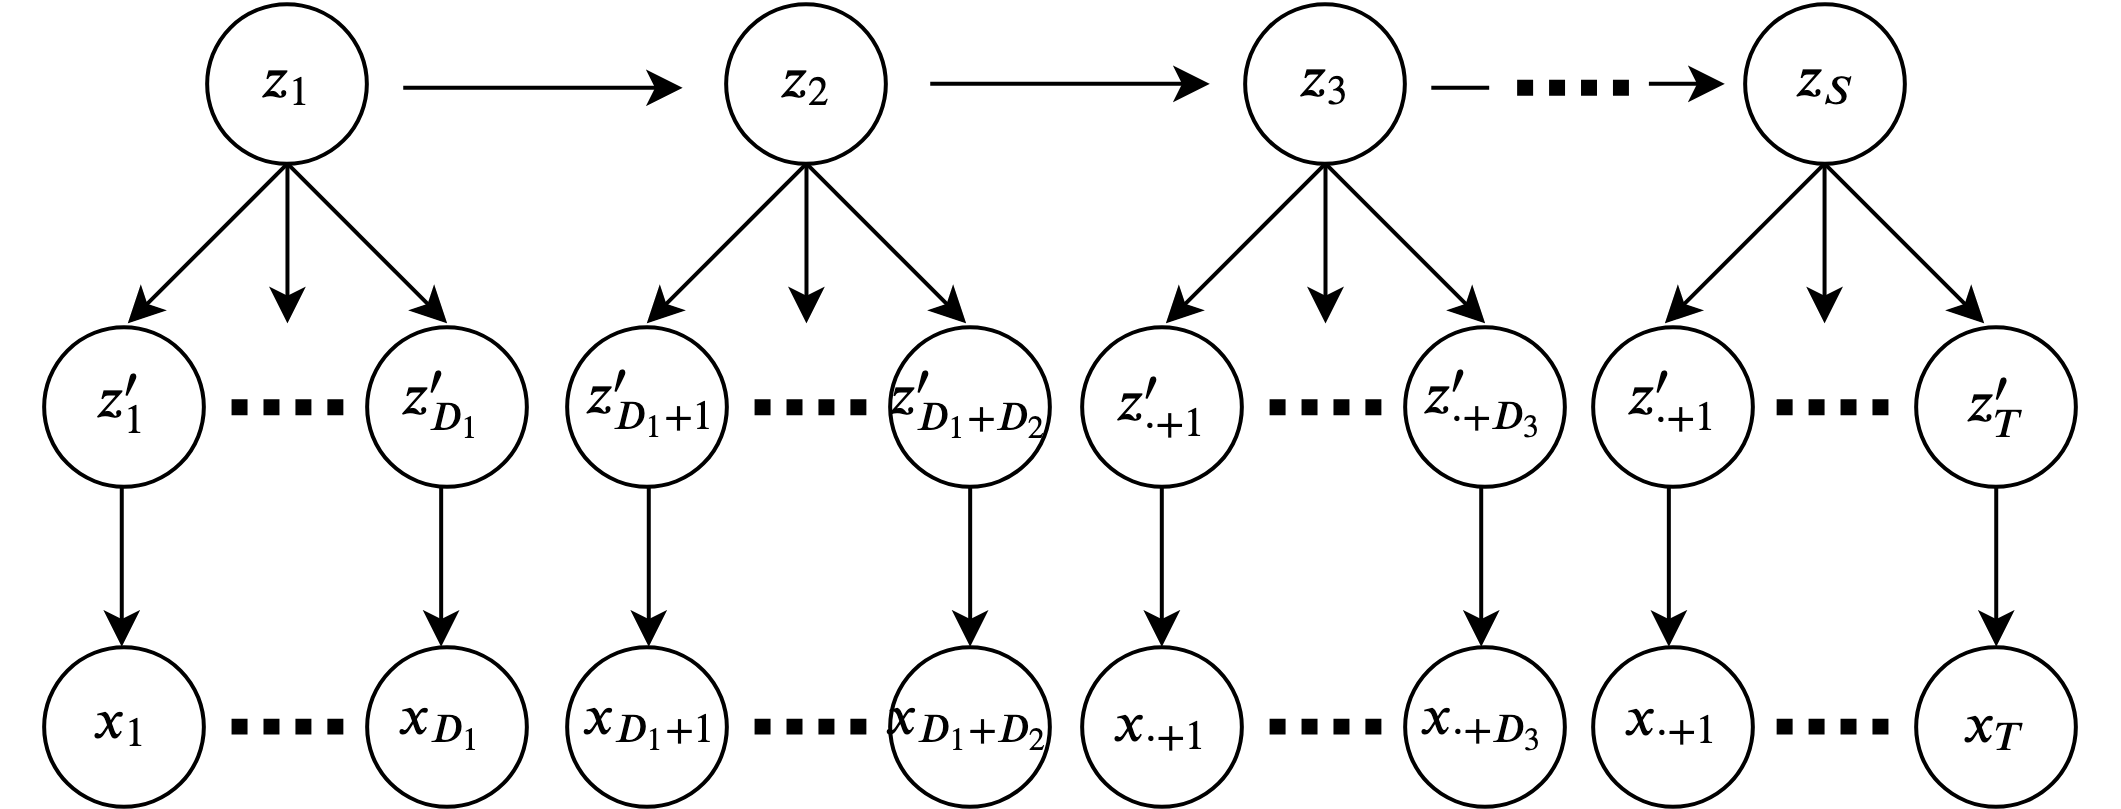
\includegraphics[scale=0.15]{images/hsmm2.png}
    \caption{HSMM where super state transitions are Markovian, while emissions associated with each state follow some explicit duration distribution.}
    \label{fig:hsmm}
    \end{figure}
\end{frame}

\begin{frame}
    \frametitle{HDP-HMM}
    A HDP-HMM$(\gamma, \alpha, H)$ model is governed by:
    \begin{itemize}
      \item $\beta_k \coloneqq \beta_k'\cdot \prod_{i=1}^{k-1} (1-\beta_i')$ where $\beta_i' \overset{\text{i.i.d}}{\sim} Beta(1,\gamma)$
      \item $\pi_k \overset{\text{i.i.d}}{\sim} DP(H(\beta), \alpha)$ for $k = 1, \dots, \infty$ where $\beta = \{\beta_k\}_{k=1}^{\infty}$
      \item $z_t \sim \pi_{z_{t-1}}$
      \item $x_t \sim h(\theta_{z_t})$ where $\theta_{k} \sim H$ for $k = 1, \dots, \infty$
    \end{itemize}
    Interpretation:
    \begin{itemize}
        \item $\gamma, \alpha > 0$: concentration parameters, $H$: base distribution of Dirichlet process (DP)
        \item $\{\beta_k\}_{k=1}^{\infty}$: stick-breaking process with parameter $\gamma$
        \item $\{\pi_k \}_{k=1}^{\infty}$: transition distributions drawn from DP, $h(\theta_{z_t})$: observation distributions drawn from $H$
        \item Each state $z_t$ is drawn from $\pi_{z_{t-1}}$, and each observation $x_t$ is drawn from $h(\theta_{z_t})$
    \end{itemize}
\end{frame}

\begin{frame}
    \frametitle{HDP-HSMM}
    HDP-HSMM is an augmentation of the HDP-HMM to \textbf{include duration distributions}. The main difference is that durations $D_s$ are drawn from base distribution $G$ and sub-states $z'_{t_{s}:t'_{s}}$ are then set to the corresponding super-state $z_{s}$ where $t_{s}:t'_{s}$ are sequence indices
    \begin{itemize}
      \item $\beta_k \coloneqq \beta_k'\cdot \prod_{i=1}^{k-1} (1-\beta_i')$ where $\beta_i' \overset{\text{i.i.d}}{\sim} Beta(1,\gamma)$
      \item $\pi_k \overset{\text{i.i.d}}{\sim} DP(H(\beta), \alpha)$ for $k = 1, \dots, \infty$ where $\beta = \{\beta_k\}_{k=1}^{\infty}$
      \item $z_s \sim \tilde{\pi}_{z_{s-1}}$
      \item $D_s \sim g(\omega_{z_s})$ where $\omega_k \sim G$ for $k = 1, \dots, \infty$
      \item $z'_{t_{s}:t'_{s}} = z_s$ where $t_{s} = \sum_{s' < s} D_s + 1$ and $t'_{s} = t_{s} + D_s - 1$
      \item $x_{t_{s}: t'_{s}} \overset{\text{i.i.d}}{\sim} h(\theta_{z'_t})$ where $\theta_{k} \sim H$ for $k = 1, \dots, \infty$
    \end{itemize}
\end{frame}

\begin{frame}
    \frametitle{Illustration of HDP-HSMM}
    \begin{figure}[H]
    \centering
    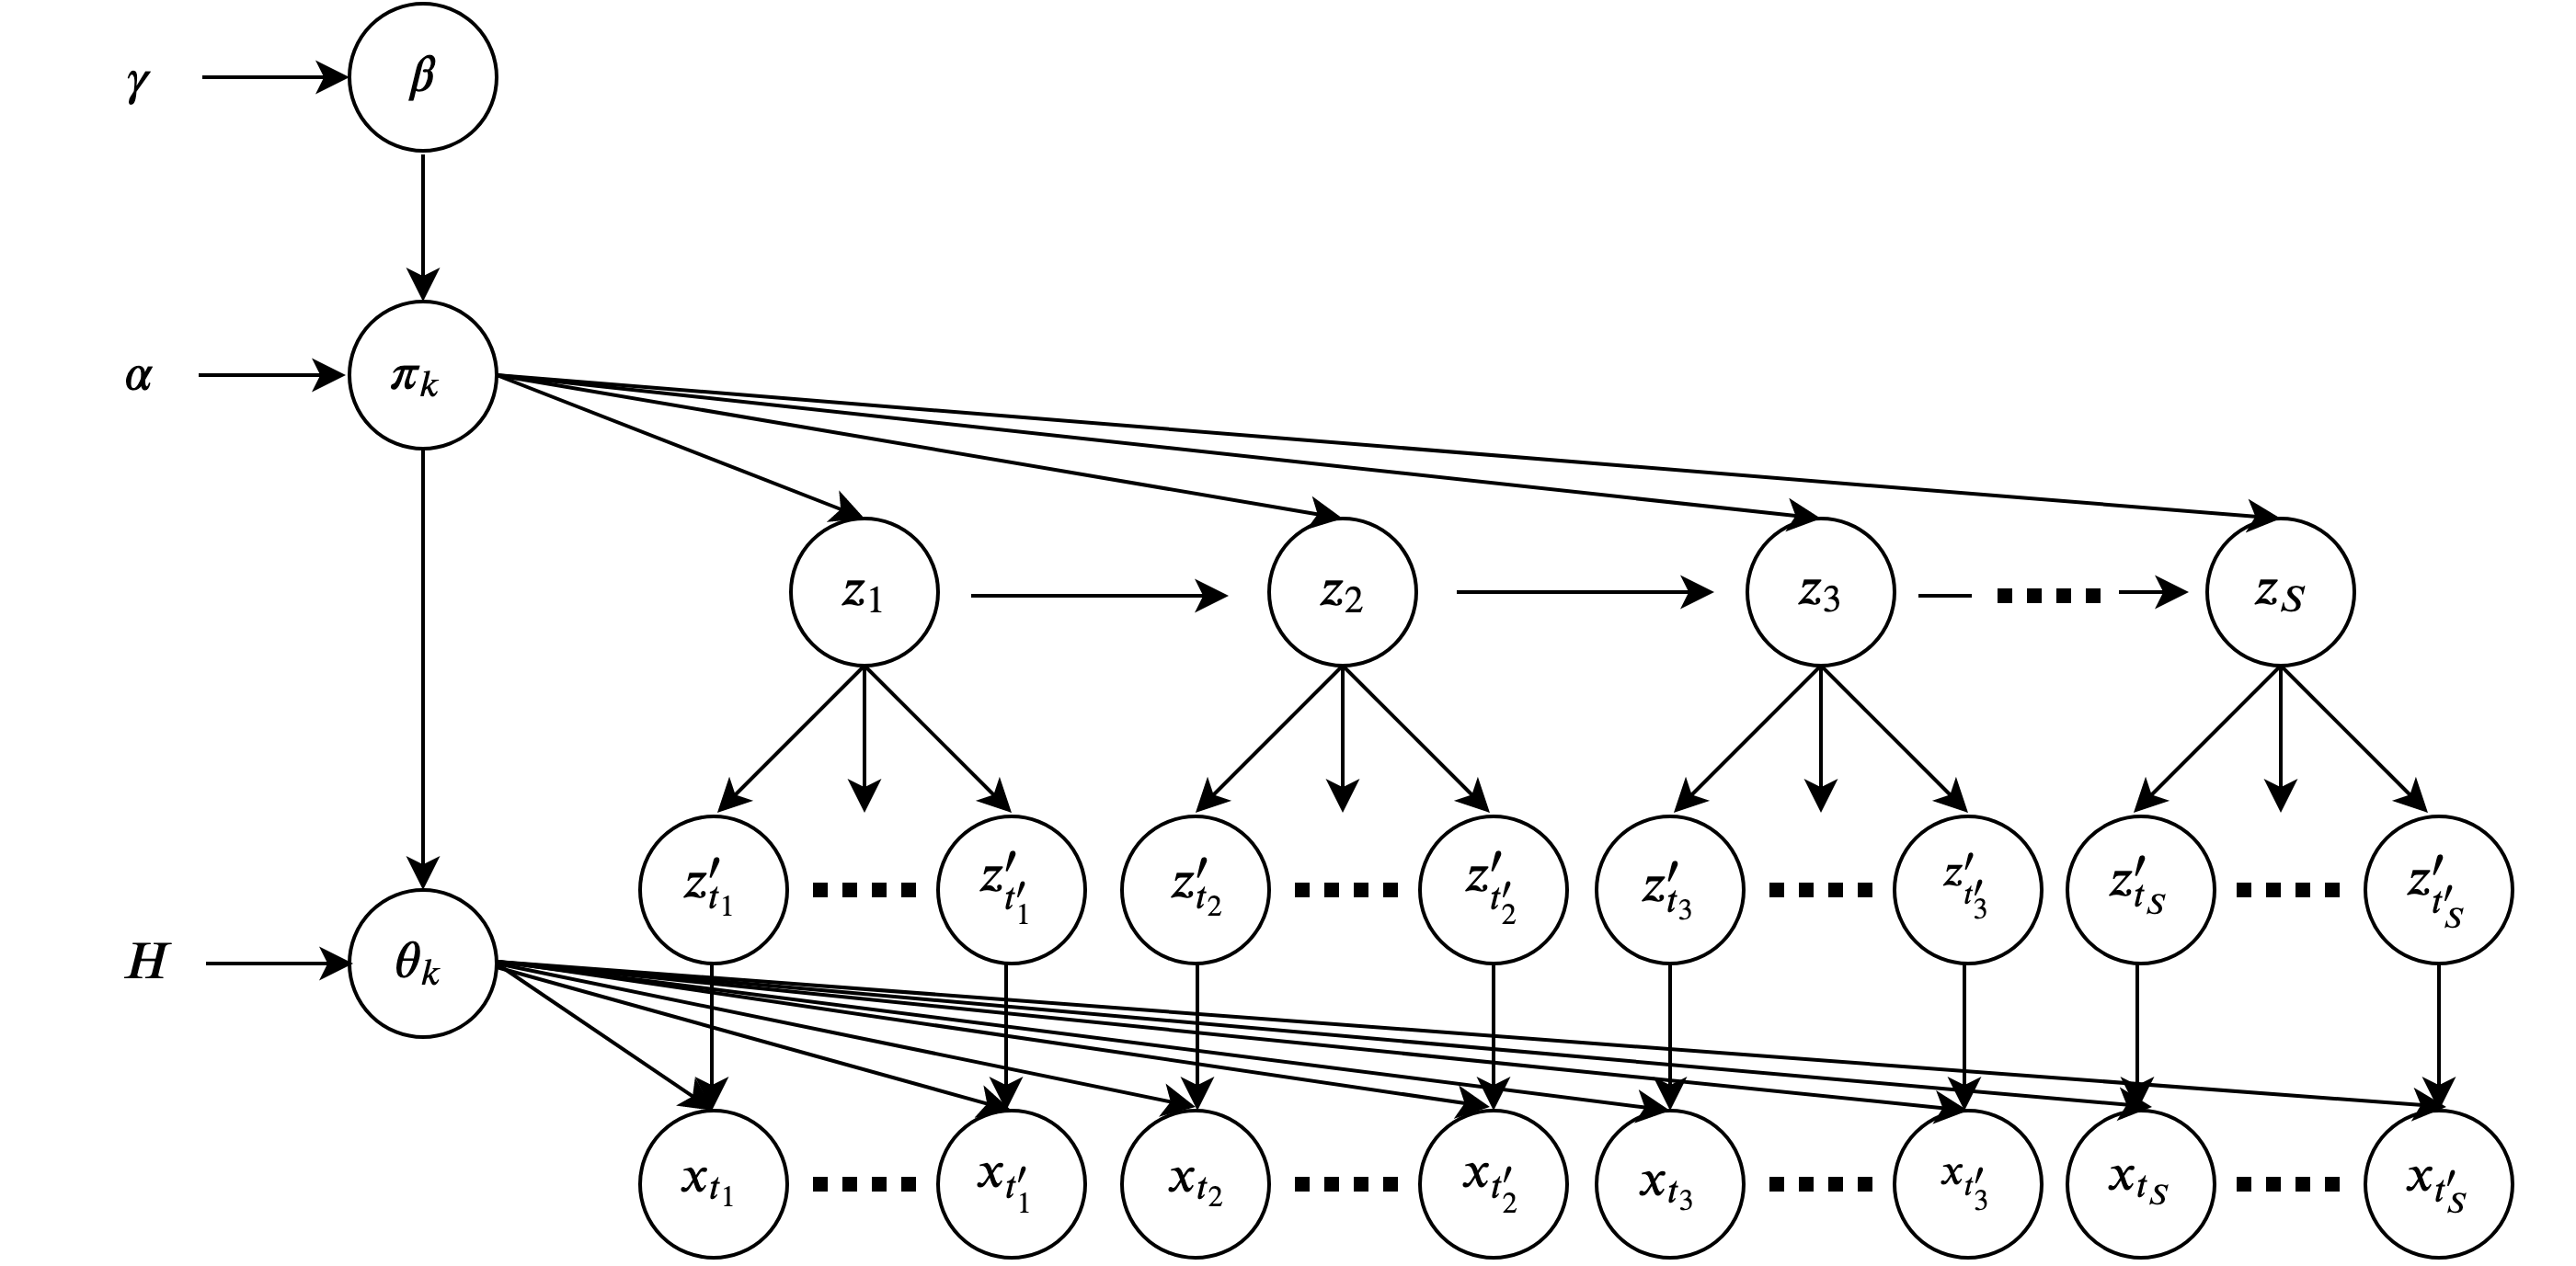
\includegraphics[scale=0.12]{images/hdphsmm.png}
    \caption{HDP-HSMM incorporates a HDP component into a HSMM}
    \label{fig:hdphsmm}
    \end{figure}
\end{frame}

\begin{frame}
    \frametitle{Data Generation - GridWorld Settings}
        \begin{itemize}
            \item Grid Size: 5x5
            \item States: The observation at each state is Gaussian with mean $\mu$ as the true identity of the state, $\sigma$ is constant across all states
            \item Obstacles: Different formation of obstacles indicate states that cannot be visited by the agent
        \end{itemize}

        \newcommand{\addmapa}{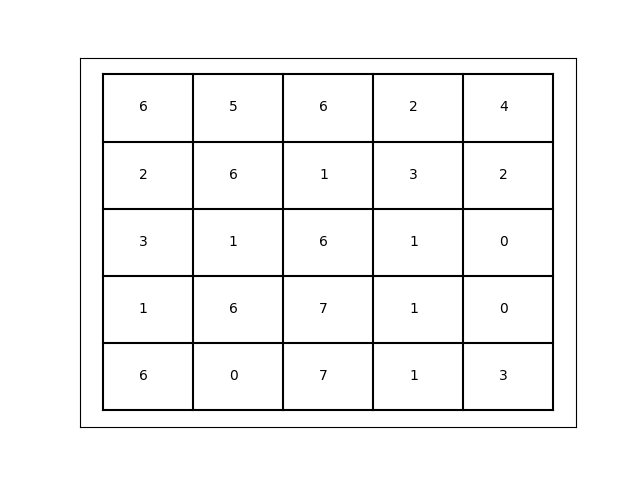
\includegraphics[width=10em]{data/Model1/5x5;4;free.png}}
        \newcommand{\addmapb}{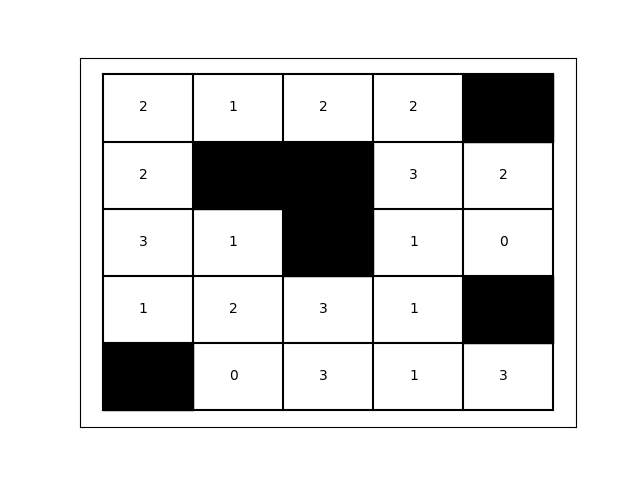
\includegraphics[width=10em]{data/Model2/5x5;4;6box.png}}
        \newcommand{\addmapc}{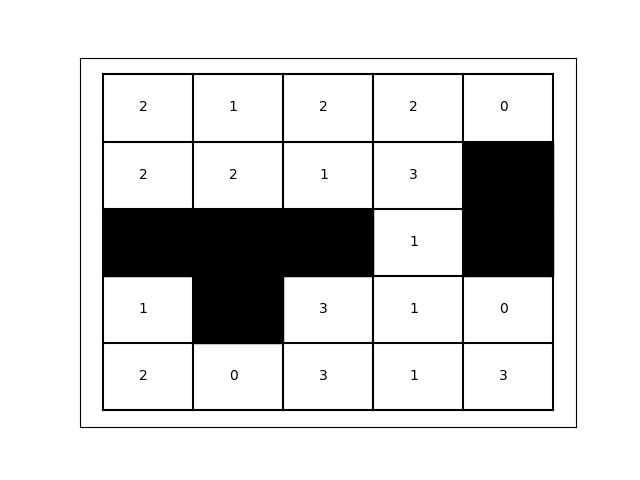
\includegraphics[width=10em]{data/Model3/5x5;4;6sep.png}}
        \newcolumntype{C}{>{\centering\arraybackslash}m{8em}}
        \begin{table}[H]
        \sffamily
        \centering
        \begin{tabular}{l*3{C}@{}}
        \addmapa \addmapb \addmapc \\
        \end{tabular}
        \caption{GridWorld Maps}
        \end{table}
\end{frame}

\begin{frame}
    \frametitle{Data Generation - Agent Motion}
    \begin{itemize}
    \item \textbf{Purely Random}: Uniform transition probability over all states (including current state). This setting satisfies the Markov property, as each realization of a future state is independent from the history of all previous states
    \item \textbf{Traditional Markov}: The state sequences are generated using a fixed transition matrix -- the probability of transitioning from one state to the next is constant as the sequence is generated. This setting also satisfies the Markov property
    \item \textbf{Sticky Transitions}: The HDP-HSMM specializes in inferring observations when the underlying motion is presumed to be "sticky". Specifically, a sticky process is one where transition probabilities correspond to an agent's elapsed duration in the same state. In our implementation, the probability of staying in the same state decreases geometrically with the duration, and resets upon entering a new state
    \end{itemize}
\end{frame}

\begin{frame}
    \frametitle{Results}
    \begin{itemize}
        \item Results
    \end{itemize}
\end{frame}


\begin{frame}
    \frametitle{References}
    \begin{itemize}
        \item [1] Johnson, M.J.\ \& Willsky, A.S.\ (2013) Bayesian Nonparametric Hidden Semi-Markov Models, {\it Journal of Machine Learning Research 14 (2013)},
        pp.\ 673--701. Cambridge, MA: MIT Press.
    \end{itemize}
\end{frame}

\end{document}
